\documentclass[11pt, a4paper]{article}

\usepackage[czech]{babel}
% \usepackage[IL2]{fontenc} % pro iso8859-2
\usepackage[utf8]{inputenc}   % pro unicode UTF-8

\newcommand{\Author}{Tomáš Báča}
\newcommand{\Title}{Řídicí deska multikopter}
\newcommand{\Acronym}{Acronym}
\newcommand{\WorkPackage}{WorkPackage}
\newcommand{\DocName}{Technický manuál}
\newcommand{\Subject}{\WorkPackage - \DocName}
\newcommand{\Keywords}{mobile robotics}
\newcommand{\Date}{11/07/2011}
\newcommand{\DOCVersion}{0.1}

\pdfoutput=1
\documentclass[a4paper,12pt,titlepage, twoside]{article}


\usepackage[english]{babel}
\usepackage[utf8]{inputenc}
\usepackage{amssymb,amsmath}
\usepackage{algorithm,algpseudocode}
\usepackage[title,titletoc]{appendix}
\usepackage{latexsym}
\usepackage{a4wide}
\usepackage{color} 
\usepackage{indentfirst}
\usepackage{graphicx}       %%% graphics for dvips
\usepackage{fancyhdr}
\usepackage{longtable}
\usepackage{pifont}
\usepackage{makeidx}
\usepackage{lastpage}
\usepackage{multirow}
\usepackage{dcolumn} 
\usepackage{epstopdf}
\usepackage{url}
\usepackage{listings}
\usepackage{caption}
\usepackage{subcaption}
\usepackage{relsize}
\usepackage{pdfpages}
\usepackage{rotating}
\usepackage{natbib}
\usepackage{cite}
\usepackage{booktabs}
\usepackage[table,xcdraw]{xcolor}

\newcommand{\Author}{Jiří Fiedler}
\newcommand{\Title}{MAV communication protocol}
\newcommand{\Acronym}{Acronym}
\newcommand{\WorkPackage}{WorkPackage}
\newcommand{\DocName}{MAV communication protocol}
\newcommand{\Subject}{\WorkPackage - \DocName}
\newcommand{\Keywords}{mobile robotics}
\newcommand{\Date}{11/05/2015}
\newcommand{\DOCVersion}{1.0}

% European layout (no extra space after `.')
\frenchspacing

% nastavení výstupu
\def\nothtml{}  					%%% \nothtml is defined if not processed with latex2html
\usepackage[                		%%% hyper-references for ps2pdf
bookmarks=true,%                   	%%% generate bookmarks ...
breaklinks=true,%                  	%%% breaks lines, but links are very small
hypertexnames=false,%              	%%% needed for correct links to figures
colorlinks=false,%
urlcolor=blue
]{hyperref}           				%%% blue instead of cyan URLS
\hypersetup{
pdfcreator  = {LaTeX with hyperref package},
pdfproducer = {dvips + ps2pdf},
colorlinks=false,
pdfborder={0 0 0},
}

\hypersetup{  
pdfauthor={\Author},
pdftitle={\Title - \Acronym},
pdfsubject={\Subject},
pdfkeywords={\Keywords}}

% úpravy vzhledu stránek
\setlength{\headheight}{18pt}			%%% drobně odsadí hlavičku
\renewcommand{\footrulewidth}{0.4pt}  	%%% horizontal line in footer
\fancyhead[R]{} 						%%% umaže pravou stranu hlavičky

\newcommand{\jed}[1]{\ensuremath{~\mathrm{#1}}} %příkaz pro sazbu fyzikálních jednotek
\newcommand{\dd}[1]{\ensuremath{\mathrm{d}#1}} %příkaz pro sazbu diferenciálu
\newcommand{\EE}[1]{\ensuremath{ \cdot 10^{#1}}} %příkaz pro sazbu *10^x

\newcommand{\pd}[2]{\ensuremath{\frac{\partial #1}{\partial #2}}} %parc. derivačka

\begin{document}

\begin{titlepage}

\begin{center}

\textsc{\LARGE České vysoké učení technické v Praze }\\[1.0cm]
\textsc{\LARGE Fakulta elektrotechnická }\\[1.0cm]
\textsc{\large Skupina inteligentní a mobilní robotiky }\\[0.5cm]

% Title
%\HRule \\[5.0cm]
{ \huge \bfseries Technický manuál\\[0.5cm] řídicí deska multicopter }\\[1.0cm]
%\HRule \\[1.5cm]

% Author and supervisor
\large
\textsc{\Author}

\vfill

\end{center}

\end{titlepage}

\newpage

\tableofcontents

\newpage

\setlength{\parskip}{0.35cm}
\pagenumbering{arabic}
\lhead{\emph{\leftmark}}
\rhead{}
\cfoot{}
\rfoot{\thepage$/$\pageref{LastPage}}

\section{Hardware}

\subsection{Letoun}

Letoun, jinak běžně nazývaný kvadrukoptera, je helikoptera se čtyřmi rotory. Listy mají pevný úhel náběhu a jejich tah se řídí změnu rychlosti jejich otáčení. Díky tomu je stroj konstrukčně jednoduchý a relativně odolný proti poškození (v porovnání s běžnou helikopterou). Z toho důvodu je vhodný pro experimentální použití. Stroj je napájen z Li-Poly (Lithium-Polymerová) baterie. Doba letu se pohybuje od 5 do 15 minut v závislosti na zatížení.

Samotný letoun je nestabilní systém vyžadující stabilizaci. O tu se stará výrobcem dodaná stabilizační deska FlightCTRL (Obrázek~\ref{fig:flightctrl}). Ta je osazená 3-osými MEMS gyroskopy a akcelerometry, ze kterých syntetizuje údaj o úhlu náklonu v ose Pitch a Roll. Ty potom používá pro stabilizaci letounu. Dále se deska stará o mixování vstupních signálů (výroba virtuálních vstupů) a řízení jednotlivých vrtulí.

Vstupními řídicími signály do desky jsou:
\\
\\
\textbf{THROTTLE} - Kolektivní tah všech rotorů v procentech jejich max. otáček\\
\textbf{ELEVATOR} - Náklon letounu v ose dopředu/dozadu (pitch, výškovka), úhlový rozměr\\
\textbf{AILERON} - Náklon letounu v ose doleva/doprava (roll, křidélka), úhlový rozměr\\
\textbf{RUDDER} - Rotace kolem svislé osy (yaw, směrovka), rozměr úhlové rychlosti

Vstupní signál se do FlightCTRL zavádí po jednom vodiči pomocí Pulze Poziční Modulace (PPM). V desce je stabilizace implementována formou \textbf{úhlového regulátoru}. Všechny tři osy (yaw, pitch, roll) jsou stabilizovány na nulový úhel. Před startem je vždy třeba provést kalibraci na rovné zemi, kde si jednotka nastaví referenční nulový úhel.

Srdcem FlightCTRL je mikrokontroler ATmega, software je napsán v C. Zdrojové kódy jsou k dispozici a je možnost je upravit a nahrát do kontroleru. Toho bylo využito pro získávání hodnot úhlů náklonu po seriové lince.

\begin{figure}[h]
\begin{center}
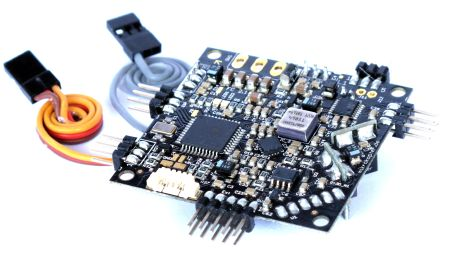
\includegraphics[width=0.4\textwidth]{fig/flightctrl.jpg}
\caption{Stabilizační deska FlightCTRL}
\label{fig:flightctrl}
\end{center}
\end{figure}

\newpage

\subsection{Řídicí deska}

Řídicí deska plní funkci komunikačního uzlu mezi moduly a malé výpočetní jednotky pro další stabilizaci a řízení letounu. Je osazena mikrokontrolerem ATmega164p s 1kb RAM a 16kb ROM (pro program). Procesor kontroleru trpí absencí FPU (floating point unit). Ke komunikaci jsou zde 2 porty UART. Programování mikrokontroleru probíhá přes SPI.

\begin{figure}[h]
\begin{center}
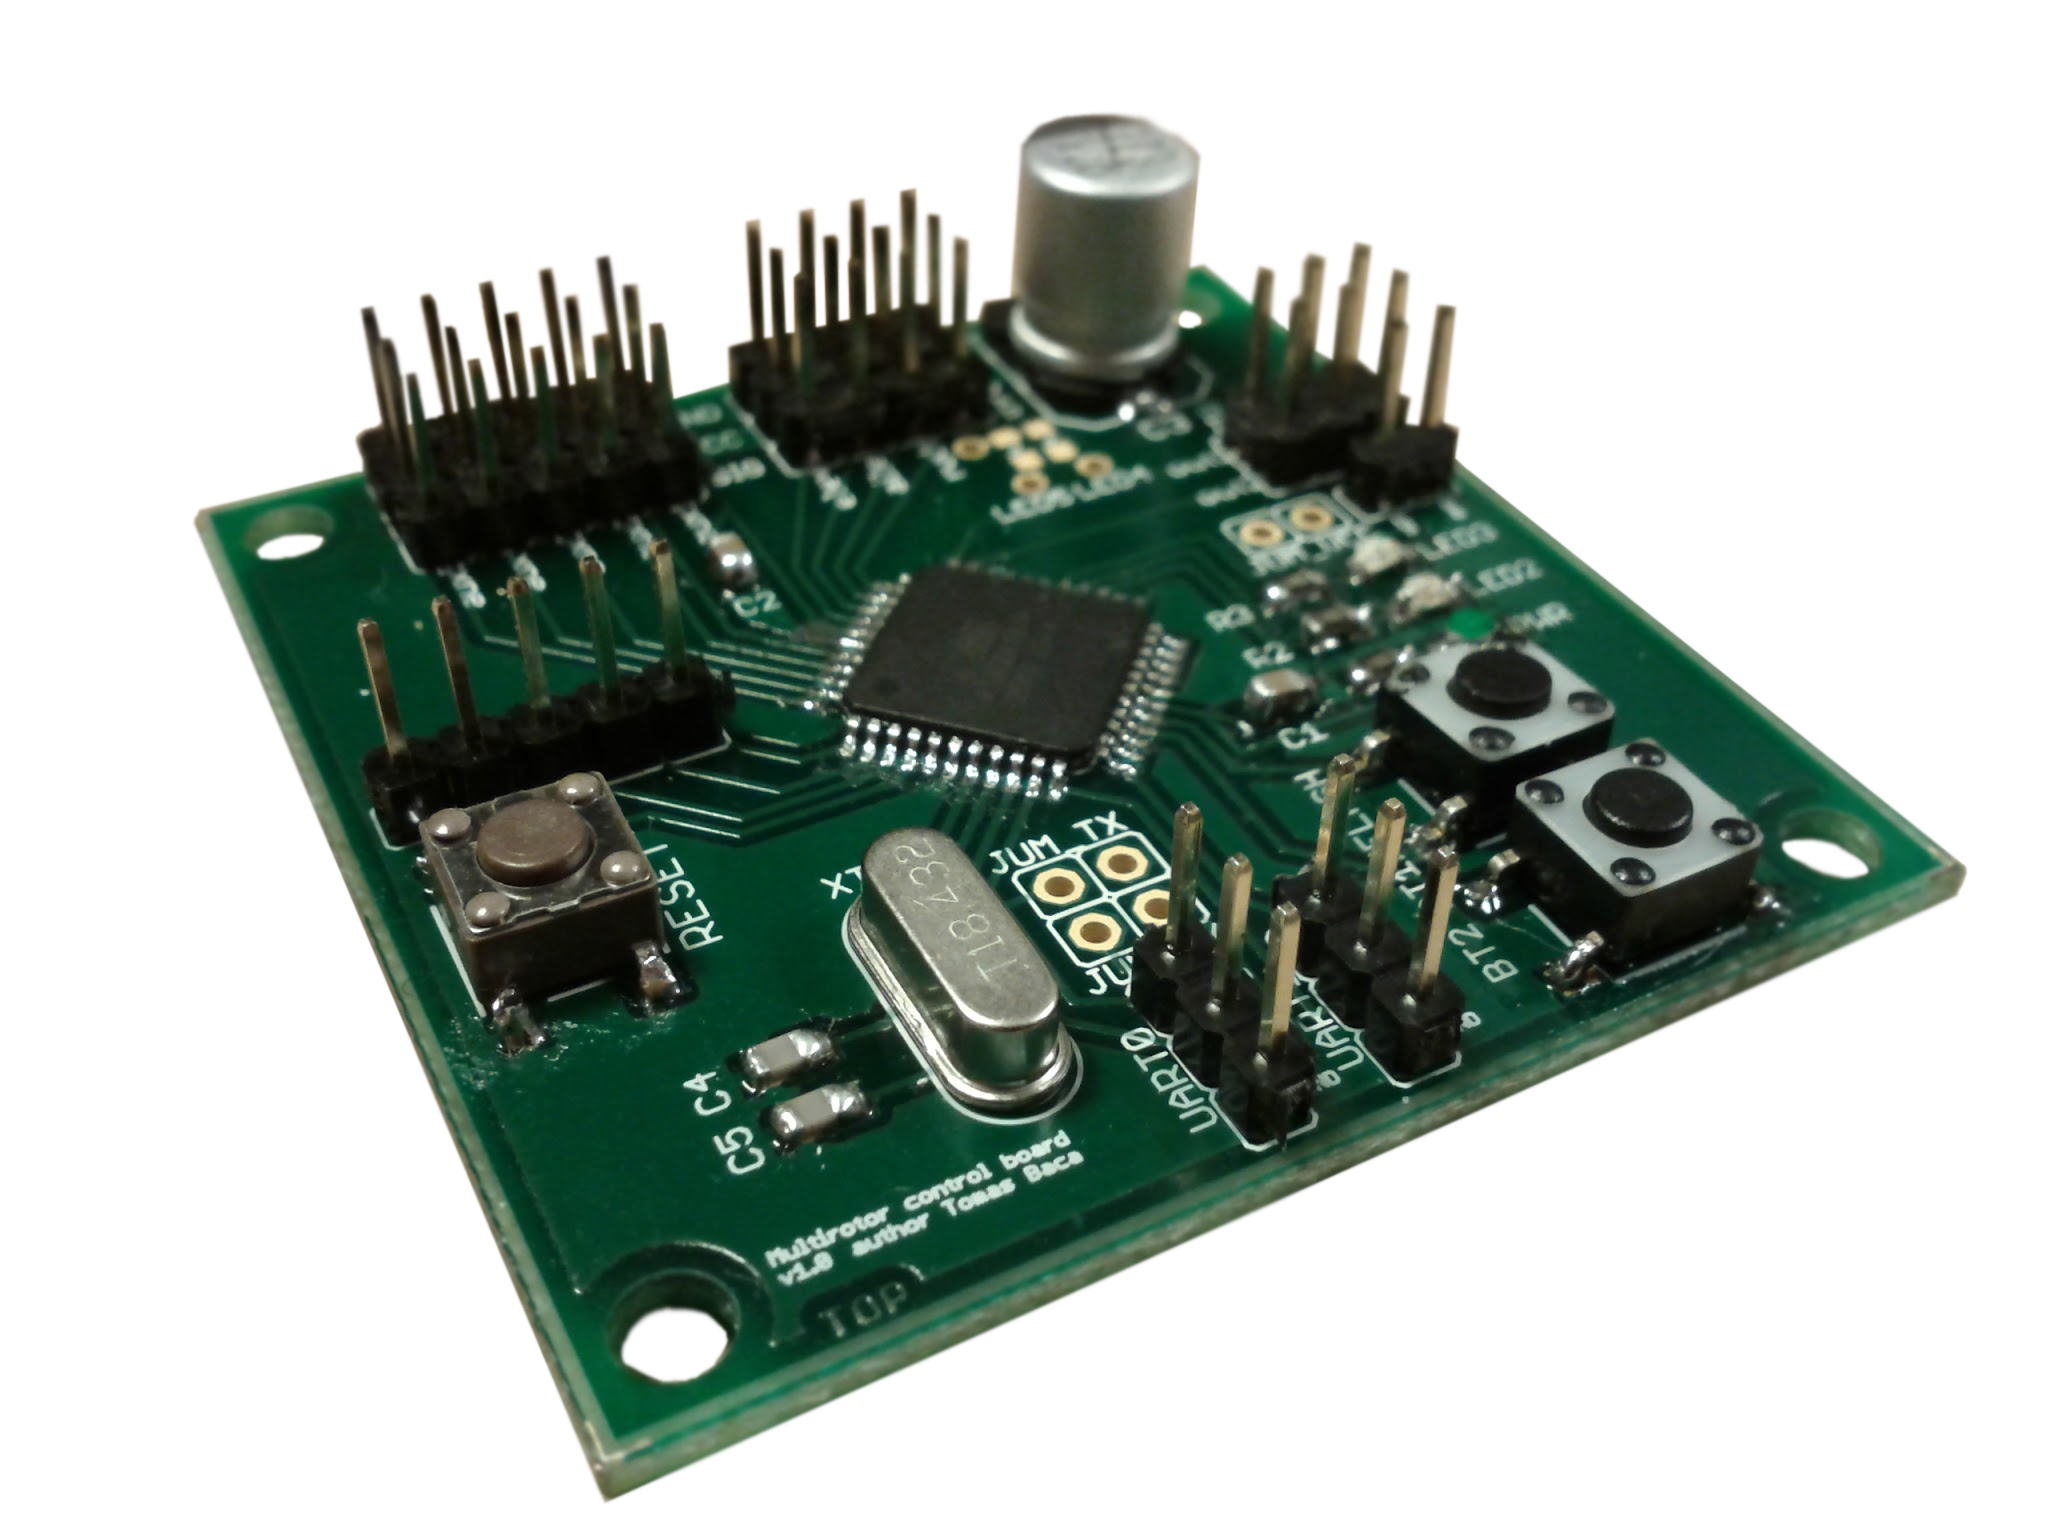
\includegraphics[width=0.4\textwidth]{fig/control_board.jpg}
\caption{Řídicí deska kvadrukoptery}
\label{fig:flightctrl}
\end{center}
\end{figure}

Deska má 9 vstupů pro Pulzně Šířkovou Modulaci (PWM). Použity jsou pro příjem signálů z RC přijímače. Dále jsou zde dva volitelné výstupy, z nichž jeden je použit pro PPM výstup do stabilizační desky FlightCTRL a druhý je volitelný.

Pro signalizaci jsou k dispozici 2 LED, žlutá a červená, třetí se dá případně připojit do volitelného výstupu.

Deska je osazena dvěma volitelnými tlačítky a jedním tlačítkem \textbf{reset}.

V minimální konfiguraci plní funkci konvertoru signálů z RC soupravy. Převádí PWM z přijímače na PPM pro FlightCTRL a umožňuje tedy ruční řízení letounu. Z důvodu bezpečnosti doporučuji vždy \textbf{zachovat majoritní vliv ručního řízení} a vyvíjené regulátory mixovat se signály z RC soupravy se značnou saturací. Zamezíte tím případné neovladatelnosti stroje. Více viz kapitola \ref{cap:controllers}.

Deska je napájena z FlightCTRL pomocí komunikačního 3-žilové kabelu. Je to standardní modelářské uspořádání s \textbf{+VCC} na prostředním pinu a \textbf{GND} a \textbf{DATA} na krajních pinech. \textbf{GND} a \textbf{+VCC} jsou na celé desce propojené. Stejným způsobem se přenáší napájení do RC přijímače. 

\subsection{Připojitelné externí moduly}

Zde uvedu další zařízení, pro která je v řídicí desce vytvořena komunikační podpora a dají se s nimi tedy relativně snadno pracovat.

\subsubsection{FlightCTRL}

V první řadě je to stabilizační deska FlightCTRL. V řídicí desce jsou funkce pro dekódování zpráv ve formátu Base64, které FlightCTRL posílá po seriové lince. Dají se tedy snadno přijímat údaje o úhlu náklonu helikoptéry a použít je dále pro řízení. Pro správnou funkčnost je však nutné mít ve FlightCTRL nahrán modifikovaný firmware, který automaticky posílá čerstvé údaje vždy, když jsou k dispozici.

\subsubsection{Počítač Gumstix}

Tento modul se obvykle stará o rozpoznávání kruhového detekčního vzoru. Dále je používán pro logování dat během letu. Modul je tvořen malým počítač s procesorem architektury ARM. Počítač disponuje wifi konektivitou, jedním UART ve funkci konzole (b.r. 115 200), druhým UART pro komunikaci s řídicí deskou (b.r. 57 600). Gumstix se automaticky připojuje na síť s SSID uKopter. V laboratoři je připraven router (bílý), který takovou síť vyrábí. IP Gumstixe je pevná - \texttt{192.168.1.103}.

Připojení přes \textbf{SSH} k bílému Gumstix: \texttt{root@192.168.1.103}, heslo prázdné

O logování dat do Gumstixe se dočtete v kapitole \ref{chap:logovani-gumstix}.

\subsection{Příprava před letem}

Po připojení napájení je potřeba provést kalibrační rutinu, bez které letoun nevzlétne. Je potřeba letoun \textbf{postavit na vodorovnou zem} a poté nastavit páčky vysílače do následujících poloh:

\begin{figure}[h]
\begin{center}
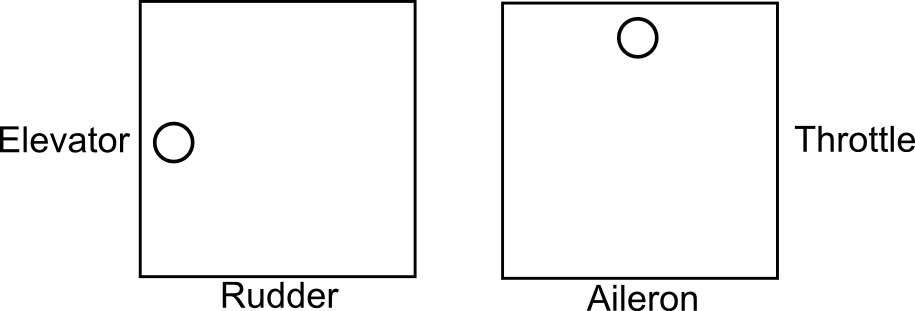
\includegraphics[width=0.6\textwidth]{fig/kalibrace1.png}
\caption{Kalibrace, část 1.}
\label{fig:flightctrl}
\end{center}
\end{figure}

Poté je potřeba letounu říci, aby si data uložil do paměti, to se provádí obdobným "gestem":

\begin{figure}[h]
\begin{center}
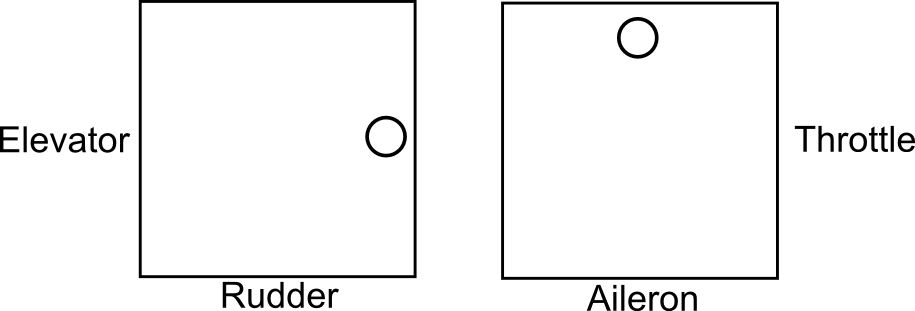
\includegraphics[width=0.6\textwidth]{fig/kalibrace2.png}
\caption{Kalibrace, část 2.}
\label{fig:flightctrl}
\end{center}
\end{figure}

\subsection{Aktivace k letu}

Pokud je letoun nakalibrovaný, je potřeba ho aktivovat (lidově "naArmovat"). To se provádí obdobným gestem. Letoun poté roztočí vrtule na minimální otáčky a je připraven k letu.

\begin{figure}[h]
\begin{center}
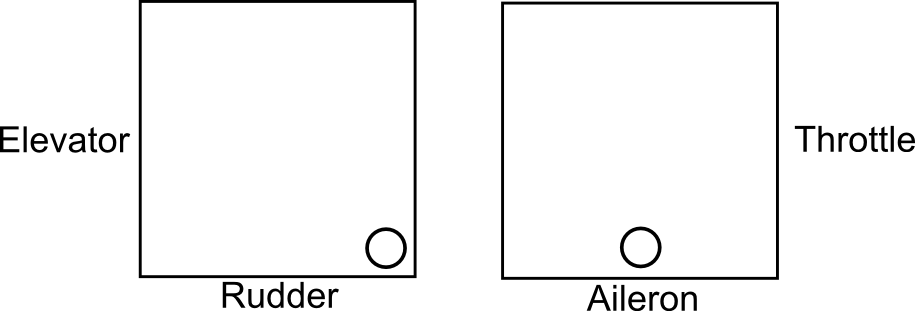
\includegraphics[width=0.6\textwidth]{fig/arm.png}
\caption{Armování letounu}
\label{fig:flightctrl}
\end{center}
\end{figure}

\subsection{Deaktivace - vypnutí}

\textbf{Velmi důležité} gesto pro disarmování letounu. Bez něj se vrtule nevypnou. Je možné zapnout automatické volání gesta řídicí jednotkou. Např. v případě vypnutí plynu na minimum.

\begin{figure}[h]
\begin{center}
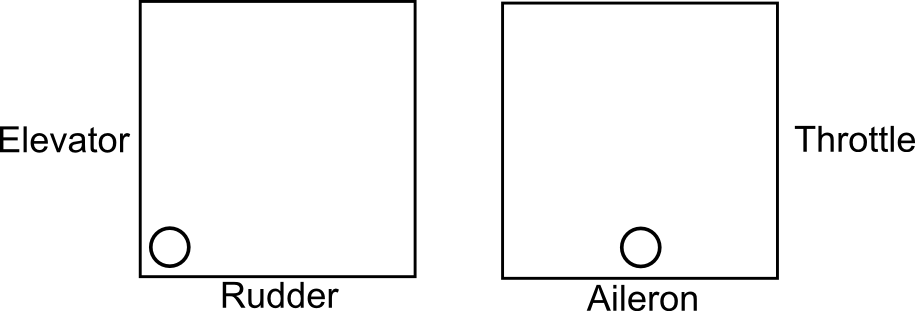
\includegraphics[width=0.6\textwidth]{fig/disarm.png}
\caption{Disarmování letounu}
\label{fig:flightctrl}
\end{center}
\end{figure}

\newpage

\section{Software}

\subsection{Struktura software}

Software pro kontroler je napsán v programovacím jazyce C. Hlavním souborem je \textbf{main.c}. Zde je hlavní smyčka programu a předpis funkcí pro přerušení přerušeními procesoru.

Většinu času tráví procesor v nekonečné smyčce ve funkci \textbf{main()}. Zde čeká na asynchronní obsluhu komunikace, nebo periodické volání řídicích funkcí apod. Je velmi důležité, aby co možná všechny výpočty, zpracování a volání funkcí probíhaly voláním z funkce \textbf{main()}. Jinak bude procesor zablokován (přerušení nebude vyvoláno, pokud procesor vykonává funkci jiného přerušení) a nebude zpracovávat komunikaci, což může vést k neovladatelnosti letounu.

Kód je strukturován pomocí podmínek preprocesoru. Pokud např. nebudete potřebovat kamerový modul s počítačem gumstix, lze v souboru \textbf{config.h} definovat \texttt{GUMSTIX\_DATA\_REVEICE} na hodnotu \texttt{DISABLED}. Všechen kód a proměnné týkající se příjmu dat a volání funkcí, s tímto modulem spojených, bude vyřazeno z kompilace.

\subsubsection{main.c}

Kód \textbf{main.c} obsahuje definici globálních proměnných. Všechny proměnné, které si mají uchovat hodnotu, musí být deklarovány zde. Všechny proměnné doporučuji definovat jako \textbf{volatile}, předejdete nečekaným problémům s jejich měnícím se obsahem.

Je zde definována funkce \textbf{main()} v níž probíhá konfigurace procesoru po spuštění a následně zanoření do nekonečné smyčky.

Dále se zde nachází obsluha přerušení, viz. Tabulka~\ref{tab:interrupts}.

V nekonečné smyčce jsou kontrolovány vlajky pro asynchronní volání funkcí. Např., poté, co přijde poslední znak zprávy z px4flow, nastaví se vlajka \textbf{px4flowDataFlag} na hodnotu 1. Ta je poté v nekonečné smyčce odchycena a jsou vykonány potřebné úkony spojené s příjmem dat - filtrace, uložení aktuálních hodnot do stavových proměnných, apod.

\begin{table}
\begin{center}
\begin{tabular}{| c | p{8cm} |}
\hline
ISR(USART0\_RX\_vect) & příjem z UART0 \\
\hline
ISR(USART1\_RX\_vect) & příjem z UART1 \\
\hline
ISR(TIMER1\_COMPA\_vect) & Komparační přerušení A k 16bit čítači. Používá se pro generování vstupního PPM signálu (start pulzu).
\newline \textbf{Neupravovat, pokud nevím, co dělám!!}\\
\hline
ISR(TIMER1\_COMPB\_vect) & Komparační přerušení B k 16bit čítači. Používá se pro generování vstupního PPM signálu (konec pulzu).
\newline \textbf{Neupravovat, pokud nevím, co dělám!!}\\
\hline
ISR(PCINT0\_vect) & Zpracování změny na vstupních PWM pinech 1..4
\newline \textbf{Neupravovat, pokud nevím, co dělám!!}\\
\hline
ISR(PCINT1\_vect) & Zpracování změny na vstupních PWM pinech 5..9
\newline \textbf{Neupravovat, pokud nevím, co dělám!!}\\
\hline
ISR(TIMER0\_OVF\_vect) & Zpracování přetečení 8bit čitače (hrubé měření času). \\
\hline
\end{tabular}
\caption{Použitá přerušení}
\label{tab:interrupts}
\end{center}
\end{table}

\subsubsection{controllers.c}\label{cap:controllers}

\textbf{controllers.c} obsahuje funkce pro řízení letounu.

\subsubsection{system.c}

\textbf{system.c} obsahuje funkce pro obsluhu kontroleru a letounu. Viz. Tabulka~\ref{tab:system.c}.

\begin{table}
\begin{center}
\begin{tabular}{| c | p{8cm} |}
\hline
initializeMCU() & Volá se jednou, po zapnutí. Provede nastavení mikrokontroleru.
\newline \textbf{Neupravovat, pokud nevím, co dělám!!}\\
\hline
enableController() & Zapne automatickou stabilizaci letounu.\\
\hline
disableController() & Vypne automatickou stabilizaci letounu.\\
\hline
armVehicle() & Provede automatické "armování" letounu. NEPOUŽÍVAT!.\\
\hline
disarmVehicle() & Provede automatické "disarmování" letounu.\\
\hline
button1check() & Kontrola stisku tlačítka 1.\\
\hline
button2check() & Kontrola stisku tlačítka 2.\\
\hline
\end{tabular}
\caption{Funkce v system.c}
\label{tab:system.c}
\end{center}
\end{table}

\subsubsection{communication.c}

\textbf{communication.c} obsahuje funkce pro obsluhu a zpracování komunikace s externími moduly. Některé funkce zpracovávají jednotlivé příchozí bajty a jsou tedy určeny pro volání zevnitř přerušení. Jiné zpracovávají celou komunikační zprávu a musejí být volání asynchronně, zevnitř smyčky, po přijetí posledního bajtu.

\begin{table}
\begin{center}
\begin{tabular}{| c | p{8cm} |}
\hline
USART0\_init() & inicializace UART0\\
\hline
USART1\_init() & inicializace UART1\\
\hline
Uart0\_write\_char() & zapíše bajt na UART0\\
\hline
Uart0\_write\_string() & zapíše string na UART1\\
\hline
atomParseChar() & zpracuje příchozí znak z "Atomového" počítače (použití pro surfnav)\\
\hline
gumstixParseChar() & zpracuje příchozí znak z Gumstixu\\
\hline
flightCtrlParseChar() & zpracuje příchozí znak z FlightCTRL stabilizační desky\\
\hline
Decode64() & dekóduje zprávu z FlightCTRL\\
\hline
parseFlightCtrlMessage() & zpracuje zprávu z FlightCTRL stabilizační desky\\
\hline
mergeSignalsToOutput() & provádí míchání signálů regulátorů a RC vysílače. \newline \textbf{Neupravovat, pokud nevím, co dělám!!}\\
\hline
px4flowParseChar() & zpracuje příchozí znak ze senzoru px4flow\\
\hline
my\_mavlink\_parse\_char() & upravená funkce z knihovny MavLink. zpracuje znak ze senzoru px4flow.\\
\hline
capturePWMInput() & měří délku PWM pulzů z RC soupravy.\newline \textbf{Neupravovat, pokud nevím, co dělám!!}\\
\hline
\end{tabular}
\caption{Funkce v communication.c}
\label{tab:communication.c}
\end{center}
\end{table}

\subsubsection{config.h}

\textbf{config.h} obsahuje direktivy preprocesoru pro konfiguraci celého firmwaru. Lze zde zapínat jednotlivé moduly (px4flow, gumstix, atomový PC, FligthCTRL) a nastavovat chování firmwaru. Dále se zde konfigurují seriové linky (jejich BAUD rate) a jejich přiřazení k modulům.

Důležité je nastavení konstant pro PWM a PPM. Jsou zde hodnoty délek pulzů (min, střední, max), délka PPM rámce a délka dělícího pulzu v PPM.

Dále je zde namapování kanálů z RC na jednotlivé PWM vstupy.

\begin{table}
\begin{center}
\begin{tabular}{| c | p{8cm} |}
\hline
FRAME\_ORIENTATION & Nastavení orientace letounu (PLUS\_COPTER, nebo X\_COPTER). Má vliv na úhly vyčítané z FlightCTRL, ty jsou vždy relativně k desce FlightCTRL. \\
\hline
GUMSTIX\_CAMERA\_POINTING & Kam míří kamera Gumstix počítače (FORWARD, nebo DOWNWARD), důležité pro rotaci souřadnic.\\
\hline
disableController() & Vypne automatickou stabilizaci letounu.\\
\hline
armVehicle() & Provede automatické "armování" letounu. NEPOUŽÍVAT!.\\
\hline
disarmVehicle() & Provede automatické "disarmování" letounu.\\
\hline
button1check() & Kontrola stisku tlačítka 1.\\
\hline
button2check() & Kontrola stisku tlačítka 2.\\
\hline
\end{tabular}
\caption{Obsah config.h}
\label{tab:config.h}
\end{center}
\end{table}

\subsection{Kompilace pro ATmega164p}

Ke kompilaci je třeba mít nainstalovaný kompilátor \textbf{avr-gcc}. Pro windows je obsažen v balíčku \textbf{WinAVR}, ke stažení na adrese \url{http://winavr.sourceforge.net/}. Pro Linux je potřeba balíčky \textbf{gcc-avr}, \textbf{binutils-avr}, \textbf{avr-libc}, \textbf{avrdude}, \textbf{gdb-avr}.

\texttt{sudo apt-get install gcc-avr binutils-avr gdb-avr avr-libc avrdude}

Pro samotnou kompilaci je přítomen soubor Makefile, který obsahuje předpis pro všechny výše popsané soubory. Výstupem kompilace je soubor \textbf{main.hex}, který je vstupním parametrem pro upload do mikrokontroleru. V Linuxu je kompilace prostá - zavoláním příkazu \texttt{make~all} ve složce se zdrojovými soubory. Ve Windows je postup stejný, pokud jste si nainstalovali výše zmíněný toolchain. Ten do windows doinstaloval program make, který umí interpretovat Makefile stejně, jako v Linuxu.

\subsection{Upload progamu do ATmega164p}

Po úspěšné kompilaci máte ve složce se zdrojovými soubory soubor \textbf{main.hex}. K jeho nahrání do kontroleru potřebujete programátor (např. USBasp) a program \textbf{avrdude}. Příkaz pro upload souboru je shodný pro Windows i Linux, pouze v Linuxu je nutné volat ho s právy superuživatele.

\texttt{avrdude -p m164P -c usbasp -U flash:w:main.hex}

\textbf{POZOR!} Před nahráváním si vždy zkontrolujte, zdali je do řídicí desky řádně přivedeno napájení. Pokud je deska bez napájení, může nahrávání firmwaru nenávratně poškodit kontroler.

\subsection{Logování letových dat do Gumstixe}\label{chap:logovani-gumstix}

Pro loggování dat z řídicí desky do Gumstixe je potřeba dvě věci. Připravit příjem na straně Gumstixe a připravit vysílání na straně řídicí desky.

\subsubsection{Strana řídicí desky}

K logování slouží funkce \texttt{debug()} v souboru \texttt{main.c}. Ve funkci připravte proměnné do formátu k odeslání (lidsky čitelný text, či jiný zápis) a předejte je funkci \texttt{uart0\_write\_string()} která zařídí jejich předání na UART. Funkce \texttt{debug()} je pravidelně volaná, typicky po vykonání výpočtů regulátorů. Ale umístění volání je vhodné zvolit individuálně na základě požadované frekvence volání a náročnosti (množství posílaných informací). V případě velkého množství posílaných dat doporučuji rozdělit data do několi separátních funkcí, které budou volané vždy v jiném průchodu hlavní smyčky.

\subsubsection{Strana Gumstixe}

V Gumstixu je nutné data ukládat na Ramdisk, z důvodu pomalé hlavní paměti počítače. Ramdisk vytvoříte zavoláním skriptu \texttt{ramdisk.sh} v domovské složce.

\begin{lstlisting}
root@192.168.1.103:~$ ./ramdisk.sh
\end{lstlisting}

Poté se přesuňte do složky ramdisku, která se nachází v \texttt{/tmp/ramdisk}:

\begin{lstlisting}
root@192.168.1.103:~$ cd /tmp/ramdisk
\end{lstlisting}

Čtení dat ze seriové linky se prování výpisem dat ze zařízení seriové linky \texttt{ttyS0}:

\begin{lstlisting}
root@192.168.1.103:/tmp/ramdisk$ cat /dev/ttyS0
\end{lstlisting}

Pokud chcete data uložit, přesměrujte výstup do souboru:

\begin{lstlisting}
root@192.168.1.103:/tmp/ramdisk$ cat /dev/ttyS0 > data.txt
\end{lstlisting}

Pokud budete mít špatné wifi spojení s Gumstixem a terminák Vám bude padat, doporučuji volat poslední příkaz na pozadí:

\begin{lstlisting}
root@192.168.1.103:/tmp/ramdisk$ nohup cat /dev/ttyS0 > data.txt &
\end{lstlisting}

Potom je samozřejmě nutné příkaz ukončit pomocí \texttt{kill}, číslo procesu zjistíte pomocí \texttt{ps -au}.

\textbf{Ihned po skončení logování} si data skopírujte z ramdisku do normálního pevného uložiště! Po vypnutí Gumstixu budou data v ramdisku ztracena.


\end{document}